% do not change these two lines (this is a hard requirement
% there is one exception: you might replace oneside by twoside in case you deliver 
% the printed version in the accordant format
\documentclass[a4paper, 11pt,titlepage,oneside,openany]{book}
\usepackage{times}


\usepackage{graphicx}
\usepackage{latexsym}
\usepackage{amsmath}
\usepackage{amssymb}
\usepackage{subfigure}
\usepackage{verbatim}
\usepackage{listings} 
\usepackage{booktabs}
\lstset{language=Python,
	basicstyle=\ttfamily\scriptsize,
	breaklines=true}    
\usepackage{glossaries}          
\usepackage{ntheorem}

% \usepackage{paralist}
\usepackage{tabularx}

% this packaes are useful for nice algorithms
\usepackage{algorithm}
\usepackage{algorithmic}

% well, when your work is concerned with definitions, proposition and so on, we suggest this
% feel free to add Corrolary, Theorem or whatever you need
\newtheorem{definition}{Definition}
\newtheorem{proposition}{Proposition}


% its always useful to have some shortcuts (some are specific for algorithms
% if you do not like your formating you can change it here (instead of scanning through the whole text)
\renewcommand{\algorithmiccomment}[1]{\ensuremath{\rhd} \textit{#1}}
\def\MYCALL#1#2{{\small\textsc{#1}}(\textup{#2})}
\def\MYSET#1{\scshape{#1}}
\def\MYAND{\textbf{ and }}
\def\MYOR{\textbf{ or }}
\def\MYNOT{\textbf{ not }}
\def\MYTHROW{\textbf{ throw }}
\def\MYBREAK{\textbf{break }}
\def\MYEXCEPT#1{\scshape{#1}}
\def\MYTO{\textbf{ to }}
\def\MYNIL{\textsc{Nil}}
\def\MYUNKNOWN{ unknown }
% simple stuff (not all of this is used in this examples thesis
\def\INT{{\mathcal I}} % interpretation
\def\ONT{{\mathcal O}} % ontology
\def\SEM{{\mathcal S}} % alignment semantic
\def\ALI{{\mathcal A}} % alignment
\def\USE{{\mathcal U}} % set of unsatisfiable entities
\def\CON{{\mathcal C}} % conflict set
\def\DIA{\Delta} % diagnosis
% mups and mips
\def\MUP{{\mathcal M}} % ontology
\def\MIP{{\mathcal M}} % ontology
% distributed and local entities
\newcommand{\cc}[2]{\mathit{#1}\hspace{-1pt} \# \hspace{-1pt} \mathit{#2}}
\newcommand{\cx}[1]{\mathit{#1}}
% complex stuff
\def\MER#1#2#3#4{#1 \cup_{#3}^{#2} #4} % merged ontology
\def\MUPALL#1#2#3#4#5{\textit{MUPS}_{#1}\left(#2, #3, #4, #5\right)} % the set of all mups for some concept
\def\MIPALL#1#2{\textit{MIPS}_{#1}\left(#2\right)} % the set of all mips



\makeglossaries

\begin{document}

\pagenumbering{roman}
% lets go for the title page, something like this should be okay
\begin{titlepage}
	\vspace*{2cm}
  \begin{center}
   {\Large Hyperpartisan News Detection\\}
   \vspace{2cm} 
   {Bachelor Thesis\\}
   \vspace{2cm}
   {presented by\\
    Larissa Strauch \\
    Matriculation Number 1518629\\
   }
   \vspace{1cm} 
   {submitted to the\\
    Data and Web Science Group\\
    Prof.\ Dr.\ Ponzetto\\
    University of Mannheim\\} \vspace{2cm}
   {Juli 2019}
  \end{center}
\end{titlepage} 

% no lets make some add some table of contents
\tableofcontents
\newpage

\listofalgorithms

\listoffigures

\listoftables

\newglossaryentry{tfidf}
{
	name=TF-IDF,
	description={Term Frequency-Inverse Term Frequency}
}
\newglossaryentry{bert}
{
	name=BERT,
	description={Bidirectional Encoder Representations from Transformers}
}
\newglossaryentry{cbow}
{
	name=CBOW,
	description={Continous Bag of Words}
}


\printglossaries %in cmd for printing: makeindex -s BA.ist -t BA.glg -o BA.gls BA.glo

% evntuelly you might add something like this
% \listtheorems{definition}
% \listtheorems{proposition}

\newpage


% okay, start new numbering ... here is where it really starts
\pagenumbering{arabic}

\chapter{Introduction}

\section{Problem Statement}
 
 

\section{Contribution}

 

\section{Related Work}


\chapter{Data}
\label{cha:theory}


\section{Data Description}
 The given data, on which we want to build our model on, was provided by zenodo.org as part of SemEvals Task 4 [Link zu Task hinzufügen]and consists of 2 independent datasets, which in turn have been divided into a GroundTruth-, Training- and Validation set.
 
 \noindent The first dataset, recognizable by the term 'byPublisher', reflects the publisher's general bias set forth by BuzzFeed journalists or MediaBiasFastCheck.com beforehand. It consists of a total of 750,000 items, of which 600,000 belong to the Training- and 150,000 to the Validation set.
 
 \noindent In return, the second dataset, recognizable by the term 'byArticle', was scrapped by crowdsourcing at hand and therefore consists of only 645 items without a Validation set.\\
 \\
 The GroundTruth dataset was provided as an XML File and consists of the features 'article url', 'labeled-by', 'id' and 'hyperpartisan'. In addition, the GroundTruth dataset scrapped 'byPublisher' contains the feature 'bias'.
\begin{itemize}
	\item Article-url: Contains the article's url.
	\item Labeled-by: Reflects whether the respective article was labeled 'byPublisher' or 'byArticle'.
	\item Id: Allocates each article a unique id.
	\item Hyperpartisan: Displays whether the particular article has been labeled as hyperpartisan or not.
	\item Bias: Divides the publisher's bias into 'left', 'left-center', 'least', 'right-center' and 'right'.
\end{itemize}
 The Training dataset was as well provided as an XML file and contains the contents of the website of the respective article. In addition, it consists of the features 'article title' 'published-at' and 'id'.
\begin{itemize}
	\item Article title: Represents the articles title.
	\item Published-at: Specifies the published date.
	\item Id: A unique id, which is the same as the corresponding entry in the GroundTruth dataset.
\end{itemize}

 \noindent The given Data has been cleaned in advance, therefore no additional steps were necessary.\\ 
 The main focus of the datasets is on the Hyperpartisan feature, on which we want to classify the articles as this thesis progresses.
 

\subsection{Dataset labelled by Publisher}
As mentioned above, this dataset consists of a total of 750,000 articles and is divided into a training record consisting of 600,000 articles and a validation set consisting of 150,000 articles. Summarizing these two sets of data, a total of 375,000 were labelled as 'Hyperpartisan' and 375,000 were not – which corresponds to a 50:50 distribution. But even individually, this distribution does not change. 
\begin{figure}[h]
	\centering
	%Arbeit:
	%includegraphics[width=0.5\textwidth]{C:/Users/lastrauc/Documents/Git/ThesisPaper/Pictures/Hypeprartisan_LabeledByPublisher.png}
	%PC:
	\includegraphics[width=0.5\textwidth]{C:/Users/Laris/Documents/Bachelorarbeit/Git/ThesisPaper/Pictures/Hypeprartisan_LabeledByPublisher.png}
	%Lap Top:
	%\includegraphics[width=0.5\textwidth]{C:/Users/Larissa/Documents/Uni/Bachelorarbeit/Git/ThesisPaper/Pictures/Hypeprartisan_LabeledByPublisher.png}
	\caption{Distribution of as Hyperpartisan labelled articles by publisher}
	\label{fig:example}
\end{figure}

\noindent This dataset also includes the feature 'bias', which informs you about the general bias of the publisher. All 375,000 Hyperpartisan labelled all are assigned to either the left or right sectors, but none are right-centre, least or left-centre and are again 50:50 distributed.


\noindent The other 50\% are split between the remaining bias, with 'Least' owning the largest share at 37\%.\\
The publicity data is distributed over the years 1964-2018, with most of the data coming from 2012-2018.
\begin{figure}[h]
	%Arbeit:
	%\subfigure[Distribution of Bias]{\includegraphics[width=0.5\textwidth]{C:/Users/lastrauc/Documents/Git/ThesisPaper/Pictures/Bias_Distribution.png}}
	%\subfigure[Distribution of Bias]{\includegraphics[width=0.5\textwidth]{C:/Users/lastrauc/Documents/Git/ThesisPaper/Pictures/Distribution_PublishedAt_Publisher_AllYears.png}}  
	%PC:
	\subfigure[Distribution of Bias]{\includegraphics[width=0.5\textwidth]{C:/Users/Laris/Documents/Bachelorarbeit/Git/ThesisPaper/Pictures/Bias_Distribution.png}} 
	\subfigure[Distribution of publishing years]{\includegraphics[width=0.5\textwidth]{C:/Users/Laris/Documents/Bachelorarbeit/Git/ThesisPaper/Pictures/Distribution_PublishedAt_Publisher_AllYears.png}} 
	%Lap Top:
	%\subfigure[Distribution of Bias]{\includegraphics[width=0.5\textwidth]{C:/Users/Larissa/Documents/Uni/Bachelorarbeit/Git/ThesisPaper/Pictures/Bias_Distribution.png}}
	%\subfigure[Distribution of publishing years]{\includegraphics[width=0.5\textwidth]{C:/Users/Larissa/Documents/Uni/Bachelorarbeit/Git/ThesisPaper/Pictures/Distribution_PublishedAt_Publisher_AllYears.png}}
\end{figure}


\subsection{Dataset labelled by Article}

The dataset labelled by Article is a little different to the larger one labelled by publisher. Here the articles were individually labelled by hand. Accordingly, the distributions of this dataset are completely different. This becomes quiet obvious if we look at how the distribution of the Hyperpartisan labelled articles is here.
\begin{figure}[h]
	%Arbeit:
	%\subfigure[Distribution of Hyperpartisan labelled articles]{\includegraphics[width=0.5\textwidth]{C:/Users/lastrauc/Documents/Git/ThesisPaper/Pictures/Hypeprartisan_LabeledByArticle.png}} 
	%\subfigure[Distribution of publishing years]{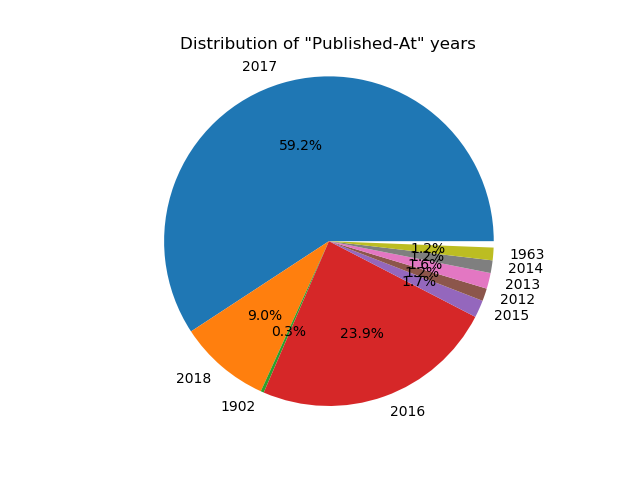
\includegraphics[width=0.5\textwidth]{C:/Users/lastrauc/Documents/Git/ThesisPaper/Pictures/Distribution_Published-At_ByArticle}} 
	%PC:
	\subfigure[Distribution of Hyperpartisan labelled articles]{\includegraphics[width=0.5\textwidth]{C:/Users/Laris/Documents/Bachelorarbeit/Git/ThesisPaper/Pictures/Hypeprartisan_LabeledByArticle.png}} 
	\subfigure[Distribution of publishing years]{\includegraphics[width=0.5\textwidth]{C:/Users/Laris/Documents/Bachelorarbeit/Git/ThesisPaper/Pictures/Distribution_PublishedAt_Article.png}} 
	%Lap Top:
	%\subfigure[Distribution of Hyperpartisan labelled articles]{\includegraphics[width=0.5\textwidth]{C:/Users/Larissa/Documents/Uni/Bachelorarbeit/Git/ThesisPaper/Pictures/Hypeprartisan_LabeledByArticle.png}} 
	%\subfigure[Distribution of publishing years]{\includegraphics[width=0.5\textwidth]{C:/Users/Larissa/Documents/Uni/Bachelorarbeit/Git/ThesisPaper/Pictures/Distribution_PublishedAt_Article.png}}
\end{figure}
\noindent Here we can see that there is no 50:50 distribution left. Only 36.9\% were defined here as Hyperpartisan as shown in figure 2.4.\\
\noindent Moreover, in this dataset, the distribution of publication data is not mainly from the years 2012-2018, but in 2016-2018, with the largest number of articles dating back to 2017 at just under 60\% as we can see in figure 2.5. Altogether all 645 articles date from the years 1902-2018.

\section{Data Analysis}

Hyperpartisan means "extremely partisan; extremely biased in favor of a political party." [definition]. This often materializes in relation to significant political events. As a result, in the following chapter, I will discuss in detail the direct link between the various features, especially the correlations between publication dates and label, as well as the connections between publisher and label.\\
\begin{table}[h]
\begin{minipage}{.4\textwidth}
		\begin{tabular}{ccc}
		\toprule
		Publisher & Amount \\
		\midrule
		The Gateway Pundit & 17 \\
		
		OpsLens & 14 \\
		
		RealClearPolitics & 13 \\
		
		New York Post & 10 \\
		
		Salon & 8 \\
		\bottomrule
	\end{tabular}
	\caption{Publsihers who have published more than 7 Hyperpartisan Articles}
\end{minipage}
\hspace{0,8cm}
\begin{minipage}{.4\textwidth}
		\begin{tabular}{ccc}
		\toprule
		Publisher & Bias & Amount \\
		\midrule
		Fox Business & Left & 96175 \\
		
		CounterPunch & Left & 39832 \\
		
		Mother Jones & Left & 36730 \\
		
		Truthdig & Left & 25056 \\
		
		Daily Wire & Right & 18570 \\
		\bottomrule
	\end{tabular}
	\caption{Publishers who have published more than 10.000 Hyperpartisan articles}
\end{minipage}
\end{table}

\noindent The two tables 2.1 and 2.2 list the publisher who produced the highest amount of Hyperpartisan articles in the respective dataset. To keep track, only those publishers who have published more than 7 Hyperpartisan articles in the dataset 'labelled by article' and who have published more than 10.000 hyperpartisan articles in the dataset 'labelled by publisher' are included in the tables. However, a problem here is the dataset 'Labelled by Publisher', since this record, as previously described, has been labelled by the overall bias of the publisher. Meaning, for the further development, we can not include the publishers, since each article of a publishing house has the same label. What I would like to discuss later, however, is the connection between whether or not one of the publishers listed in Table 2.2 published more articles in important political years.


\section{Data Preparation}
In order to be able to work with the existing data in the further course of this project, several preprocessing steps are necessary. In the preprocessation phase of my bachelor's thesis, the data therefore went through the following steps:
\begin{enumerate}
	\item Read the XML files. 
	\item Filter out the important information.
	\item Merge the Groundtruth- and Training datasets into a csv file.
	\item Remove special characters and stop words.
	\item Tokenization and stemming of the datasets.
\end{enumerate}	
\noindent As a result, in the following section, I will go further into detail how I preprocessed my data.


\subsection{Read the XML files}
Since it is difficult to work with the given data in an XML format, it is necessary to bring them into a format with which it’ll be easier to work with. The particular challenge hereby is the size of the dataset labelled by publisher. A standard algorithm for reading XML files is provided by pythons DOM library ElementTree, called “ElementTree.parse”. This method returns an ElemenTree type, which "is a flexible container object, designed to store hierarchical data structures in memory" [ http://effbot.org/zone/element.htm]. Meaning, that this library forms the entire model in the memory which can pose a problem with very large files, such as ours. As a substitute,I therefore use the method “ElemenTree.iterparse”, which can process XML documents in a streaming fashion, retaining in memory only the most recently examined parts of the tree. 


\subsection{Filter out the important information}
As mentioned in Chapter 2.1 Data Description, the XML files include various features, which will play an important role in the further course of this work. It is now necessary to filter these features out of the XML format so the can be better worked with later. In order to be able to do this, we pass an algorithm the, by the iterparse method read content, which then passes through this algorithm in a double for-loop and checks for each item of an element in the content which "key" is currently processed. I then save this in an array, so that the features which have already been parsed, can be used later. \\
\noindent
\begin{minipage}{\linewidth}
\begin{lstlisting}[frame=single]
def parse_features(content, publisher):
  for event, elem in content:
    for key, value, in elem.items():
      if publisher:
        if key == 'id':
          id_array_publisher.append(str(value))
        elif key == 'published-at':
          published_at_array_publisher.append(value)
        elif key == 'title':
          title_array_publisher.append(value)
      else:
        if key == 'id':
          id_array_article.append(str(value))
        elif key == 'published-at':
          published_at_array_article.append(value)
        elif key == 'title':
          title_array_article.append(value)
      elem.clear()
\end{lstlisting}
\end{minipage}

\subsection{Merge the Groundtruth- and Training datasets into a csv file}
Since both, the Groundtruth- and Trainingdata contain important information, it is necessary to merge them into one file. I decided to use Python's library pandas to write the two files into one csv file. This, and especially Pandas, allows us to read the file more quickly as well as to access individual rows and columns of the merged file in a targeted manner.\\
\noindent
\begin{minipage}{\linewidth}
\begin{lstlisting}[frame=single]
feature_extraction.parse_features(xml_training, publisher)
groundtruth_parser.parse_groundtruth(xml_gt, publisher)
content = content_parser.parse_content(content_training)

a_id = feature_extraction.get_id_array(publisher)
published = feature_extraction.get_published_at_array(publisher)
title = feature_extraction.get_title_array(publisher)
bias = groundtruth_parser.get_bias_array(publisher)
hyperpartisan = groundtruth_parser.get_hyperpartisan_array(publisher)

columns = {"ArticleID": a_id,
           "PublishedAt": published,
           "Title": title,
           "Bias": bias,
           "Content": content,
           "Hyperpartisan": hyperpartisan}

tf = Pd.DataFrame(columns)
tf = tf[['ArticleID','Published', Title','Bias','Content','Hyperpartisan']]
tf.to_csv(titlecsv,encoding='utf-8',index=False)
\end{lstlisting}
\end{minipage}

\subsection{Remove special characters and stop words}
Now that we have merged both files and written them into a csv file, we need to remove special characters and stop words. Especially the removal of stopwords is necessary since not all words presented in a document, such as auxiliary verbs, conjunctions and articles [TextClassificationUsingMachineLearning] are useful for training a classifier. It also decreases our corpus which makes it easier to classify later on. (Warum?)\\
\noindent
\begin{minipage}{\linewidth}
\begin{lstlisting}[frame=single]
stop = stopwords.words('english')

df['Content'] = df['Content'].apply(lambda x: ''.join([item for item in x.split() if item not in stop]))
df['Title'] = df['Title'].apply(lambda x: ''.join([item for item in x.split() if item not in stop]))
df['Content'] = df['Content'].map(lambda x: re.sub(r"[^a-zA-Z0-9]+", '', x))
df['Title'] = df['Title'].map(lambda x: re.sub(r"[^a-zA-Z0-9]+", '', x))
\end{lstlisting}
\end{minipage}
\noindent Here it becomes obvious that using pandas was a good choice, as we can now specifically access the 'Content' and 'Title' columns in order to perform this step of preprocessing on only these two and not the whole file.


\subsection{Tokenization and Stemming of the datasets}
After cleaning the dataset, the words are tokenized in order to convert them into numerical vectors so that a classifier is able to work with them. Tokenization is definied as "The process of demarcating and possibly classifying sections of a string of input characters. The resulting tokens are then passed on to some other form of processing. The process can be considered a sub-task of parsing input".\\
\noindent Stemming is the procedure of reducing the word to its grammatical (morpho-syntatctic) root. The result is not necessarily a valid word of the language. For example, "recognized" would be converted to "recogniz". Still, the basic word almost always contains the very meaning of the word. Stemming is advantageous in that the algorithm used later now only has to fall back on a few different words and not many, all of which have the same meaning.\\
\\
\noindent In order to implement Stemming and Tokenization, only 2 lines of python code are necessary, due to the Pandas dataframe. \\
\noindent
\begin{minipage}{\linewidth}
\begin{lstlisting}[frame=single]
df["Content"] = df["Content"].apply(nltk.word_tokenize)
df['Content'] = df['Content'].apply(lambda x: [stemmer.stem(y) for y in x])
\end{lstlisting}
\end{minipage}
This will transform our output file in the following way:

\chapter{Text Classification Techniques}
\noindent The main process for Text Classification includes 7 steps of which the first 4 have already been performed in Chapter 2.
\begin{enumerate}
	\item Read the Document.  
	\item Tokenize Text.
	\item Stemming.
	\item Delete Stopwords.
	\item Vector Representation of the Text.
	\item Feature Selection and/or Feature Transformation.
	\item Learning Algorithm.
\end{enumerate}
As already mentioned in Chapter "Introduction", we build our classifier model by using BERT-Embeddings. To compare how our model performs, in this chapter, I will discuss the classic methods and algorithms that I have used in order to achieve this comparison. \\	

\section{Vector Representation of the Text}
In order for our classifier to be able to work with the text, we first need to transform our words into a feature vector representation. A document is a sequence of words [Text Categorization with Support Vector Machines] so a document can be presented by a One-Hot encoded vector, assigning the value 1 if the document contains the feature-word or 0 if the word does not appear in the document. [TextClassificationUsingmachineLearning]. However, using this technique for word representation, resolves in a $V \cdot V$ Matrix, as we have V-diemensional vertorr for each out of V words which can lead to huge memory issues. In addition this does not notion similiarity between words. Therefore I will go into further detail for better approaches in the next 2 subchapters.

\subsection{Term Frequency-Inverse Document Frequency}
Term frequency \textit{tf(t,d)} is a measure that denotes how frequently the term \textit{t} appears in the document \textit{d}. It is computed as follows: \\
\[
	tf(t_i, d_j)=\frac{1+log_{10}(f_{ti,gj})}{1+log_{10}(\max_{f_{t', dj}:t'\in d_j})}
\]
Inverse Doucment Frequency \textit{idf(t)} points to the assumption that the informativeness of the term \textit{t} is inversely proportional to the number of documents in the collection in which the term appears.\\
\[
	idf(t_i)=log{10}(\frac{|D|}{d' \in D : t_i \in d'})
\]
To compute the weight for the term $t_i$ within the document $d_j$ we simply multiply the \textit{TF} and \textit{IDF} components:
\[
	w_{ij}=tf(t_i, d_j)\cdot idf(t_i)
\]
Therefore, \Gls{tfidf} indicates how important a word is to a document in a collection or corpus. It is often used as a weighting factor in Information Retrieval and Text Mining. The \Gls{tfidf} value increases proportionally to the number of times a word appears in the document, but is offset by the frequency of the word in the corpus, which helps to control the fact that some words are usually more common than others. (umschreiben?) \\
\noindent \Gls{tfidf} is easy to compute. In addition, it is possible to extract the most descriptive terms, as well as to calculate the similarity between 2 terms. However, TF-IDF is based on the bag-of-words (BoW) model, which is why it disregards aspects such as text position, semantics and co-occurrence.
Many ways exist to implement \Gls{tfidf}. The one I used is as follows:\\

\noindent
\begin{minipage}{\linewidth}
\begin{lstlisting}[frame=single]
from sklearn.feature_extraction.text import CountVectorizer
from sklearn.feature_extraction.text import TfidfTransformer

def to_tf_idf(content):
	count_vect = CountVectorizer()
	tfidf_transformer = TfidfTransformer()

	content_counts = count_vect.fit_transform(content)
	content_tfidf = tfidf_transformer.fit_transform(content_counts)

	return content_tfidf
\end{lstlisting}
\end{minipage}

\noindent With "CountVectorizer" we convert a collection of text documents to a matrix of token counts. "TfidfTransformer" transforms a count matrix into a normalized \gls{tfidf} representation.
\begin{table}[t]
	\begin{minipage}{.5\textwidth}
		\begin{tabular}{ccc}
			\toprule
			Term & Average \Gls{tfidf} Weight \\
			\midrule
			trump & 0.091165 \\
			bannon & 0.065129 \\
			president & 0.061829 \\
			kimmel & 0.052415 \\
			money & 0.051647 \\
			americans & 0.049132 \\
			people & 0.047342 \\
			obamacare & 0.042512 \\
			wall & 0.042117 \\
			control & 0.039068 \\
			\bottomrule
		\end{tabular}
		\caption{Top 10 terms by average \Gls{tfidf} weight (By Article)}
	\end{minipage}
	\hspace{0,8cm}
	\begin{minipage}{.5\textwidth}
		\begin{tabular}{ccc}
			\toprule
			Terms & Average \Gls{tfidf} Weight \\
			\midrule
			balls & 0.057251 \\
			said & 0.051183 \\
			medicare & 0.047450 \\
			martin & 0.046519 \\
			school & 0.044264 \\
			university & 0.043572 \\
			says & 0.042079 \\
			trump & 0.041235 \\
			carrier & 0.040903 \\
			degree & 0.040704 \\
			\bottomrule
		\end{tabular}
		\caption{Top 10 terms by average \Gls{tfidf} weight (By Publisher)}
	\end{minipage}
\end{table}


\subsection{Word Embeddings}
Word Embeddings are based on the approach of Harris Distributional Hypothesis from 1951, which states, that words that occur in the same contexts tend to have similar meanings. \\
\noindent A Word Embedding provides a word vector for every word. It takes a word and gives it a vector representation by extracting features from that word within the context that word appears in and assigns it a place within a vector space. Two similar word will occupy places which are close to each other within that vector space whereas words that are different, will have locations much further away from each other. This allows computation of distance calculation, which is why, for example, we're able to tell which word is similar to "small" in the same sense as "biggest" is similar to "big". We simply have to compute the vector \textit{X}, which is equal to $Vector_{biggest}-Vector_{big}+Vector_{small}$ and then we find the word which is closest to \textit{X} in the vector space, measured by cosine distance. [Efficient Estimation of Word Representations in Vector Space]
\subsubsection{Word2Vec}
Word2Vec is a "2-Model Architecture for computing continuous vector representations of words from very large dataset" [Efficient Estimation of Word Representations in Vector Space] that creates an n-dimensional vector space in which each word is represented as a vector. Word2Vecs 2 learning models are the \gls{cbow} and Skip-Gram-Model (Figure 3.1).\\
\\
\noindent \gls{cbow} uses the context word to predict the target word. The input is a one-hot encoded vector. The weights between the input layer and the output layer can be represented by a $V \cdot N$ matrix \textit{W} where each row of \textit{W} is the \textit{N}-dimensional vector representation $v_W$ of the input word [word2vec Parameter Learning Explained]. The hidden-layer \textit{h} is computed by multiplying the one-hot encoding vector of the input word $w_I$ with the weight matrix \textit{W}.
\[
	h=W_{(k, \cdot)}^{T}:=v_{w_I}^{T}
\] 
Next we have another weight matrix $W'={w'_{ij}}$ which is an $N \cdot V$ matrix. With these weights we can finally compute a score $u_j$ for each word in the vocabulary
\[
	u_{j}={v'}_{w_j}^{T}h
\] where ${v'}_{w_j}$ is the \textit{j}-th column of the matrix \textit{W'}. Afterwards we use \textit{softamax}, which is a log-linear classification model, to obtain the posterior distribution of words.
\[
	p(w_j|w_I)=y_j=\frac{exp(u_j)}{\sum_{j'=1}^V exp(u_{j'})}
\] \\
\\
\noindent In contrast to the \gls{cbow} model,  Skip-Gram uses the target word to predict the context words. The input is still a one-hot encoding vector, the hidden layers definition stays the same as in the \gls{cbow} model, each output is still using the same hidden layer to output matrix as in the \gls{cbow} model $p(w_{c,j}=w_{O,c}|w_I)=y_{c,j} = p(w_j|w_I)=y_j$ and the function for $u_j=u_{c,j}$ stays the same. However in the output layer, we are now outputting \textit{C} multinomial distributions. \\
\\
\noindent Learning the output vector is expensive.
\begin{figure}[t]
	\centering
	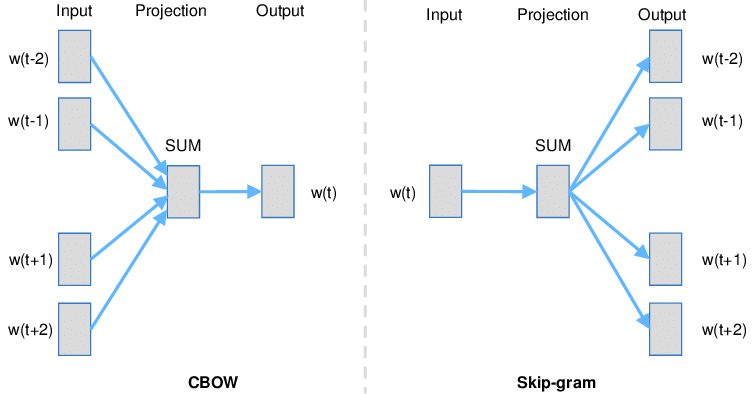
\includegraphics[width=0.5\textwidth]{C:/Users/Laris/Documents/Bachelorarbeit/Git/ThesisPaper/Pictures/Cbow_skip.png}
		\caption{The CBOW and Skip-Gram architectures}
	\label{fig:CBOW and Skip-Gram architectures}
\end{figure}
\section{Feature Selection and/or Feature Transformation}
\section{Learning Algorithms}
\subsection{SVM}
\subsection{Multinomial Naive Bayes Classifier}
\subsection{Random Forest Classifier}
\subsection{Logistic Regression Classifier}
\newpage


\pagestyle{empty}


\section*{Ehrenw\"ortliche Erkl\"arung}
Ich versichere, dass ich die beiliegende Master-/Bachelorarbeit ohne Hilfe Dritter
und ohne Benutzung anderer als der angegebenen Quellen und Hilfsmittel
angefertigt und die den benutzten Quellen w\"ortlich oder inhaltlich
entnommenen Stellen als solche kenntlich gemacht habe. Diese Arbeit
hat in gleicher oder \"ahnlicher Form noch keiner Pr\"ufungsbeh\"orde
vorgelegen. Ich bin mir bewusst, dass eine falsche Er- kl\"arung rechtliche Folgen haben
wird.
\\
\\

\noindent
Mannheim, den 31.08.2014 \hspace{4cm} Unterschrift


\end{document}
